\documentclass[11pt,a4paper]{article}

\usepackage[utf8]{inputenc}
\usepackage[T1]{fontenc}
\usepackage{lmodern}
\usepackage[provide=*,spanish]{babel}
\usepackage{amsmath,amssymb,booktabs,tabularx,array,graphicx,geometry,xcolor}
\usepackage{hyperref,url}
\Urlmuskip=0mu plus 1mu

% El guion se compila desde presentation/. Los resultados numéricos proceden
% del mismo archivo generado que consume el informe para evitar cifras distintas.
% Archivo generado automáticamente; no editar a mano.
\newcommand{\ResultsDate}{2026-09-04}
\newcommand{\PoissonSurvival}{35.2}
\newcommand{\PolarSurvival}{77.8}
\newcommand{\PoissonCILow}{30.7}
\newcommand{\PoissonCIHigh}{40.1}
\newcommand{\PolarCILow}{73.4}
\newcommand{\PolarCIHigh}{81.6}
\newcommand{\PoissonMeanTime}{64.694}
\newcommand{\PolarMeanTime}{83.666}
\newcommand{\PoissonPeak}{14.220}
\newcommand{\PolarPeak}{11.225}
\newcommand{\SurvivalDifference}{-42.5}
\newcommand{\SurvivalDiffLow}{-48.8}
\newcommand{\SurvivalDiffHigh}{-35.8}
\newcommand{\McNemarP}{1.697\times 10^{-28}}
\newcommand{\PeakDifference}{2.995}
\newcommand{\PeakP}{7.007\times 10^{-39}}
\newcommand{\TestCount}{18}
\newcommand{\SmallestNominalP}{0.1716}
\newcommand{\ExponentialKSP}{0.1863}
\newcommand{\NormalKSP}{0.9236}
\newcommand{\AcceptanceRate}{0.7765}
\newcommand{\AcceptanceP}{0.1716}
\newcommand{\LognormalMeanP}{0.7158}
\newcommand{\CountDispersionP}{0.3464}
\newcommand{\CountChiP}{0.7887}
\newcommand{\UniformKSP}{0.3006}
\newcommand{\UniformSerialP}{0.4918}
\newcommand{\LcgKSP}{0.8062}
\newcommand{\LcgSerialP}{0.6986}
\newcommand{\ControlUniformityP}{0.9999}
\newcommand{\ControlKSP}{1.0000}
\newcommand{\ControlRunsP}{<10^{-16}}
\newcommand{\ControlLjungP}{<10^{-16}}
\newcommand{\ControlSerialP}{<10^{-16}}
\newcommand{\PoissonMicros}{0.040}
\newcommand{\PolarMicros}{0.147}
\newcommand{\PolarNormalKSP}{0.1337}
\newcommand{\BoxMullerKSP}{0.3288}
\newcommand{\PolarNormalMicros}{0.105}
\newcommand{\BoxMullerMicros}{0.051}
\newcommand{\PolarRejectedPercent}{21.8}
\newcommand{\NormalMethodWinner}{Box-Muller}
\newcommand{\PolarMethodScore}{3.908}
\newcommand{\BoxMullerMethodScore}{4.800}
\newcommand{\BothSurvive}{99}
\newcommand{\OnlyPoisson}{42}
\newcommand{\OnlyPolar}{212}
\newcommand{\BothFail}{47}

\graphicspath{{../assets/}}
\geometry{margin=2.1cm}

\definecolor{outbreakdark}{HTML}{0B100D}
\definecolor{outbreakgreen}{HTML}{4F7A32}
\definecolor{outbreakpale}{HTML}{EDF4E9}
\definecolor{outbreakamber}{HTML}{B96B16}

\hypersetup{
  pdftitle={Guion de exposicion - Outbreak Stochastic Survival Lab},
  pdfauthor={Grupo 1 - Seccion 30},
  colorlinks=true,
  linkcolor=outbreakgreen,
  urlcolor=outbreakgreen
}
\setlength{\parindent}{0pt}
\setlength{\parskip}{0.45em}

\newcommand{\slidecue}[4]{%
  \subsection*{\textcolor{outbreakgreen}{Diapositiva #1 --- #2}\hfill
  \normalfont\small #3}
  \noindent\colorbox{outbreakpale}{\parbox{\dimexpr\textwidth-2\fboxsep}{#4}}
  \vspace{0.45em}}
\newcommand{\stage}[1]{\textbf{\textcolor{outbreakamber}{Acción:}} \emph{#1}\par}
\newcommand{\handoff}[1]{\vspace{0.4em}\textbf{Transición:} \emph{#1}\par}
\newcommand{\keyidea}[1]{%
  \noindent\colorbox{outbreakdark}{\parbox{\dimexpr\textwidth-2\fboxsep}{%
  \color{white}\textbf{Idea central:} #1}}}

\begin{document}
\hypersetup{pageanchor=false}
\begin{titlepage}
\pagecolor{outbreakdark}\color{white}\centering
\vspace*{0.5cm}
{\small\bfseries UNIVERSIDAD DEL VALLE DE GUATEMALA\par}
\vspace{0.2cm}
{\small CC2017 --- Modelación y Simulación · Sección 30\par}
\vspace{0.75cm}
{\Huge\bfseries GUION DE EXPOSICIÓN\par}
\vspace{0.15cm}
{\LARGE\bfseries\textcolor{outbreakgreen!45!white}{OUTBREAK}\par}
{\large Stochastic Survival Lab\par}
\vspace{0.55cm}
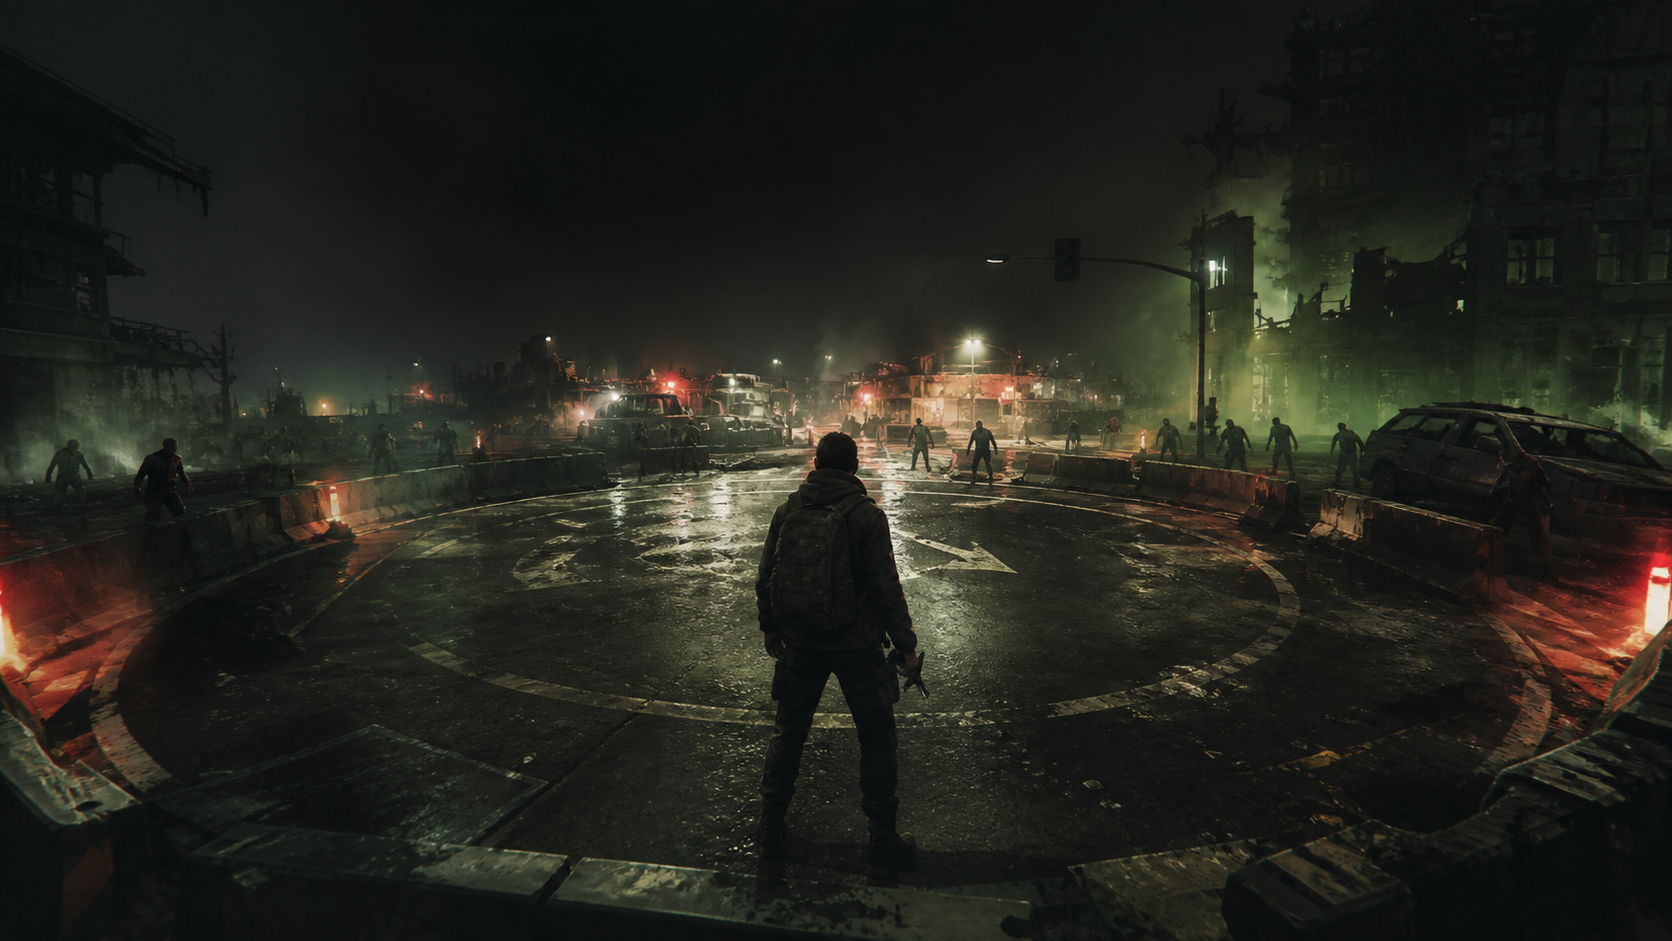
\includegraphics[width=0.80\textwidth]{outbreak-command-center.png}
\vfill
{\normalsize Duración objetivo: 18 minutos + preguntas\par}
\vspace{0.35cm}
{\small
Pablo Daniel Barillas Moreno · Jorge Palacios\par
Adrián Ricardo González Muralles\par
Andrés Rafael Chivalán · Javier Andrés Chen\par}
\vspace{0.35cm}
{\small Agosto de 2026\par}
\end{titlepage}
\hypersetup{pageanchor=true}
\nopagecolor\color{outbreakdark}

\section*{Uso y reparto}

El texto dentro de cada recuadro puede decirse casi literalmente. Las
indicaciones marcadas como \textbf{Acción} no se leen; describen señalamientos,
cambios de diapositiva y pasos de la demostración. Cada integrante debe ensayar
su transición y conocer la respuesta corta a las preguntas finales.

\begin{center}
\small
\begingroup
\setlength{\tabcolsep}{4.5pt}
\begin{tabularx}{\textwidth}{>{\bfseries}p{3.7cm}p{2.1cm}p{1.25cm}X}
\toprule
Integrante & Diapositivas & Tiempo & Responsabilidad principal \\
\midrule
Pablo Daniel Barillas Moreno & 1--5 & 3:20 & Problema, objetivos, flujo y Poisson \\
Jorge Palacios & 6--10 & 3:20 & Inversa, Polar, lognormal y fuentes \\
Adrián Ricardo González Muralles & 11--15 & 3:30 & Validación, Box--Muller, combate y arquitectura \\
Andrés Rafael Chivalán & 16--20 & 3:30 & 3D, Monte Carlo, resultados y sensibilidad \\
Javier Andrés Chen & 21--26 & 4:20 & Interpretación, verificación, demo y cierre \\
\bottomrule
\end{tabularx}
\endgroup
\normalsize
\end{center}

\keyidea{Se comparan dos procesos de llegada y, por separado, dos algoritmos
para generar la misma normal. Polar no se presenta como otro proceso de Poisson.}

\section{Pablo Daniel Barillas Moreno}

\slidecue{1}{Portada}{25 s}{
``Buenas tardes. Somos el Grupo 1 de la sección 30 y presentamos
\textbf{Outbreak: Stochastic Survival Lab}. Modelamos un sistema real de
software: el subsistema de aparición y balance de enemigos de un videojuego de
supervivencia. La narrativa es un apocalipsis zombi; el problema técnico es
cuándo aparecen entidades aleatorias y cómo esa presión afecta el resultado.''
}

\slidecue{2}{Problema y pregunta}{35 s}{
``Una aparición exactamente cada dos segundos es predecible. En un sistema
estocástico conocemos una intensidad media, pero no el instante del siguiente
evento. Preguntamos cómo cambian la congestión y la supervivencia al modificar la
tasa y la forma de los tiempos entre llegadas.''
}

\slidecue{3}{Objetivos}{35 s}{
``Nuestro objetivo fue construir una simulación reproducible que conectara
variables aleatorias continuas con consecuencias observables. Generamos y
validamos variables, comparamos métodos y procesos, estimamos supervivencia con
Monte Carlo y comunicamos el resultado mediante una app, una escena 3D,
gráficos, informe y presentación.''
}

\slidecue{4}{Flujo del sistema}{40 s}{
\stage{Recorrer el diagrama de izquierda a derecha.}
``Los uniformes alimentan los interarribos; al acumularlos obtenemos el
calendario de apariciones. Cada enemigo recibe atributos reproducibles, se
mueve y participa en el combate. El estado produce supervivencia, tiempo,
bajas y concurrencia. Repetimos esta cadena para no concluir desde una sola
partida.''
}

\slidecue{5}{Proceso de Poisson}{50 s}{
``El modelo principal es un proceso de Poisson homogéneo. Si $N(t)$ cuenta las
apariciones hasta $t$, entonces sigue Poisson con parámetro $\lambda t$, y su
media y varianza son $\lambda t$. Esto representa tasa constante, incrementos
independientes y ausencia de memoria. En el escenario base, $\lambda=0.93$ por
segundo equivale a 55.8 llegadas por minuto.''
}

\handoff{``Jorge explicará cómo convertimos uniformes en interarribos y cómo
construimos el proceso alternativo.''}

\newpage
\section{Jorge Palacios}

\slidecue{6}{Transformada inversa}{45 s}{
``Para una exponencial, invertimos $F(x)=1-e^{-\lambda x}$. Si $U$ es uniforme,
$\Delta=-\ln(U)/\lambda$ también es exponencial, porque $1-U$ tiene la misma
distribución. Acumulamos $t_i=t_{i-1}+\Delta_i$ hasta superar el horizonte. Es
la primera técnica de generación vista en el curso.''
}

\slidecue{7}{Método polar}{45 s}{
``Marsaglia Polar propone dos uniformes en el cuadrado $(-1,1)^2$. Calculamos
$S=V_1^2+V_2^2$ y aceptamos solo si $0<S<1$. El factor
$\sqrt{-2\ln(S)/S}$ produce dos normales estándar. La aceptación teórica es
$\pi/4$, por la relación entre el área del círculo y el cuadrado.''
}

\slidecue{8}{Polar--lognormal}{40 s}{
``Una normal admite valores negativos y no puede representar segundos de
espera directamente. Usamos $\Delta=e^{\mu+\sigma Z}$ y parametrizamos $\mu$ y
$\sigma$ para que la media sea $1/\lambda$ y el CV sea 0.60. Así obtenemos
tiempos positivos y más regulares que los exponenciales, cuyo CV es uno.''
}

\slidecue{9}{Comparación justa}{40 s}{
``Poisson y Polar--lognormal conservan el interarribo medio, pero no son el
mismo proceso. Para Poisson, $E[N(T)]=\lambda T$ es exacto. Para una renovación
lognormal finita, $\lambda T$ es una referencia de largo plazo. Esa diferencia
es parte del experimento, no un error de implementación.''
}

\slidecue{10}{Fuentes aleatorias}{35 s}{
``Documentamos también ángulo, radio inicial, velocidad, HP y daño. Sus
uniformes acotadas representan heterogeneidad de balance sin valores extremos.
Separamos los flujos de llegadas y atributos para que, al comparar modelos, el
enemigo del mismo índice conserve características equivalentes.''
}

\handoff{``Adrián presentará la validación de esta cadena, la comparación
algorítmica y la forma en que el calendario llega al motor.''}

\newpage
\section{Adrián Ricardo González Muralles}

\slidecue{11}{Validación formal}{55 s}{
\stage{Señalar fuente uniforme, transformaciones y conteo en la figura.}
``La auditoría usa 18 contrastes con corrección de Holm. Primero verifica
PCG64 y un LCG propio; luego exponencial, normal, media lognormal,
independencia y aceptación; finalmente el conteo Poisson. Ninguno fue rechazado.
Un contador perfectamente uniforme funciona como control negativo: aprueba
forma, pero falla las tres pruebas de dependencia. No rechazar no demuestra que
el modelo sea verdadero; indica que la muestra no lo contradice.''
}

\slidecue{12}{Polar frente a Box--Muller}{50 s}{
``Para comparar algoritmos sin cambiar la distribución, pedimos a Marsaglia
Polar y Box--Muller generar la misma $N(0,1)$. KS no rechazó ninguno; no usamos
el tamaño del valor $p$ como ranking. Box--Muller fue más rápido y no descartó
propuestas. La matriz le asignó \BoxMullerMethodScore{} sobre cinco, frente a
\PolarMethodScore{} de Polar. Conservamos Polar por su valor didáctico como
aceptación--rechazo.''
}

\slidecue{13}{Arena y combate}{40 s}{
``Los enemigos aparecen cerca del perímetro y avanzan radialmente. El
protagonista permanece en el centro, ataca al objetivo más cercano dentro del
alcance y recibe la suma del daño de quienes llegan al contacto. La misión
termina en victoria al alcanzar $T$ con vida positiva o en derrota al llegar a cero.''
}

\slidecue{14}{Parámetros}{35 s}{
``El escenario base dura 90 segundos, usa 55.8 llegadas por minuto, CV 0.60 y
9.5 HP por segundo de daño enemigo. Esta calibración evita que ambos modelos
queden pegados al 100 por ciento. No son datos de telemetría real; por eso se
acompañan de sensibilidad y se muestran siempre las unidades.''
}

\slidecue{15}{Arquitectura}{40 s}{
``La arquitectura separa responsabilidades. \texttt{simulation.py} contiene
generadores, combate e inferencia; \texttt{visuals.py} construye gráficas y
mallas; \texttt{app.py} administra formularios, estado y caché. El informe y
la ficha leen resultados regenerables del mismo motor. Esto reduce errores de
sincronización y permite probar la matemática sin abrir Streamlit.''
}

\handoff{``Andrés mostrará la decisión 3D y la evidencia obtenida al repetir el
experimento.''}

\newpage
\section{Andrés Rafael Chivalán}

\slidecue{16}{Decisión 3D}{40 s}{
``Pygame es excelente para superficies 2D, pero un 3D requeriría OpenGL y otra
ventana. Panda3D serviría para un juego independiente. Elegimos Plotly
\texttt{Mesh3d} porque ofrece cámara y mallas dentro de Streamlit, junto con
controles, telemetría y estadística en la misma experiencia web.''
}

\slidecue{17}{Experimento Monte Carlo}{40 s}{
``Una partida es una realización. Ejecutamos 400 por modelo y estimamos la
proporción de supervivencia con intervalo de Wilson al 95 por ciento. Poisson y
Polar usan el mismo vector de semillas, de modo que la comparación es pareada y
reduce variación ajena al patrón temporal.''
}

\slidecue{18}{Resultados}{50 s}{
\stage{Señalar primero probabilidades y luego tiempos y concurrencia.}
``Poisson alcanzó \PoissonSurvival{} por ciento, con IC
[\PoissonCILow, \PoissonCIHigh]. Polar--lognormal alcanzó
\PolarSurvival{} por ciento, con IC [\PolarCILow, \PolarCIHigh]. Sus tiempos
medios fueron \PoissonMeanTime{} y \PolarMeanTime{} segundos. El resultado no
convierte a Polar en universalmente mejor: describe esta configuración.''
}

\slidecue{19}{Efectos pareados}{50 s}{
``La dirección es Poisson menos Polar. La diferencia fue
\SurvivalDifference{} puntos porcentuales, IC
[\SurvivalDiffLow, \SurvivalDiffHigh] y McNemar $p=\McNemarP$. Hubo
\BothSurvive{} pares donde ambos sobrevivieron, \OnlyPoisson{} solo Poisson,
\OnlyPolar{} solo Polar y \BothFail{} donde ambos fallaron. Poisson tuvo
\PeakDifference{} enemigos más de pico medio.''
}

\slidecue{20}{Sensibilidad}{35 s}{
``No concluimos desde una sola tasa. Las curvas repiten el experimento entre 24
y 72 llegadas por minuto. Al aumentar $\lambda$, la presión supera la capacidad
ofensiva y cae la supervivencia. La posición de la transición depende también
del CV y del balance de combate.''
}

\handoff{``Javier cerrará con la elección del modelo, las limitaciones y la
demostración en vivo.''}

\newpage
\section{Javier Andrés Chen}

\slidecue{21}{Interpretación}{45 s}{
``Poisson sigue siendo principal por su parsimonia, su costo y la relación
exacta entre conteo e interarribos cuando suponemos tasa constante,
independencia y falta de memoria. Polar aporta control del CV y demuestra que
igualar la media no iguala rachas. Mejor modelo no significa mayor
supervivencia, sino supuestos más coherentes con el sistema y los datos.''
}

\slidecue{22}{Verificación}{35 s}{
``La suite contiene 28 pruebas sobre momentos, conteos, fuentes uniformes,
control negativo, Polar, Box--Muller, reproducibilidad, geometría, semillas
pareadas, Wilson, límite temporal y calibración. También verificamos que la app
cargue, simule y ejecute la validación sin excepciones.''
}

\slidecue{23}{Supuestos y límites}{40 s}{
``La tasa es constante, el protagonista no se desplaza y los obstáculos son
visuales. Los atributos uniformes son decisiones de balance sin telemetría y
el combate usa paso finito. Las pruebas validan la generación declarada, pero
no demuestran que un modelo represente datos reales que aún no poseemos.''
}

\slidecue{24}{Conclusiones}{40 s}{
``Concluimos que los interarribos controlan directamente eventos visibles; que
igual media no implica igual concurrencia ni supervivencia; y que Monte Carlo,
intervalos y pruebas pareadas permiten comunicar incertidumbre. La separación
de motor, visuales y documentos mantiene el resultado verificable.''
}

\slidecue{25}{Demostración}{90 s}{
\stage{Cambiar a Streamlit, ya precargado.}
``Primero configuramos tasa, duración, modelo y semilla, y pulsamos
\textbf{SIMULAR MISIÓN}. En la escena 3D movemos el tiempo y la cámara. Luego
mostramos variables generadas, validación, comparación Polar--Box--Muller,
comparación de modelos y Monte Carlo. Todos los resultados dependen de entradas
visibles y pueden regenerarse.''
}

\slidecue{26}{Cierre}{20 s}{
``La incertidumbre no se elimina: se modela, se repite y se comunica con
evidencia. El código, el informe, la ficha, los datos y esta presentación están
disponibles en el repositorio. Muchas gracias; quedamos atentos a sus
preguntas.''
}

\section*{Preparación de la demostración}

Ejecutar desde \path{zombie_poisson_streamlit} antes de exponer:

\begin{verbatim}
python -m pip install -r requirements/requirements.txt
python -m streamlit run App/app.py
\end{verbatim}

\begin{enumerate}
  \item Ejecutar una misión con semilla 22193.
  \item Precargar validación, comparación y Monte Carlo para usar el caché.
  \item Abrir la presentación HTML en otra pestaña y usar pantalla completa.
  \item Mantener el informe PDF y las figuras disponibles como respaldo.
  \item Ensayar el cambio de expositor en las diapositivas 6, 11, 16 y 21.
\end{enumerate}

\section*{Preguntas probables}

\textbf{¿Por qué Poisson si Polar sobrevivió más?}

La supervivencia es una salida del balance, no una prueba de ajuste. Poisson es
principal cuando son razonables tasa constante, independencia y falta de
memoria. Polar fue más favorable porque regularizó las llegadas en este escenario.

\textbf{¿Polar es otro proceso de Poisson?}

No. Marsaglia Polar genera normales; la transformación posterior produce
interarribos lognormales y, por tanto, un proceso de renovación distinto.

\textbf{¿Por qué Box--Muller gana, pero se conserva Polar?}

La matriz compara algoritmos para la misma normal y Box--Muller fue más
eficiente en el equipo de referencia. Polar permanece porque implementa
aceptación--rechazo, uno de los métodos centrales del curso.

\textbf{¿Qué significan los valores $p$?}

Indican si la muestra contradice la hipótesis bajo un contraste. No rechazar no
demuestra verdad ni un valor $p$ mayor convierte un generador en superior.

\textbf{¿Por qué Plotly y no Pygame?}

Plotly integra mallas 3D y cámara dentro de Streamlit. Pygame es principalmente
2D; un producto 3D independiente correspondería a otro alcance.

\section*{Repositorio}

\href{https://github.com/DanielBarillasM/Proyecto-1_Grupo-1_Modelacion-y-Simulacion_Sec-30}%
{github.com/DanielBarillasM/Proyecto-1 (Grupo 1, Sección 30)}

\end{document}
